\subsection{Visual Guide to Mobile Application}
\begin{figure}[ht!]
\centering
\begin{minipage}{.5\textwidth}
  \centering
  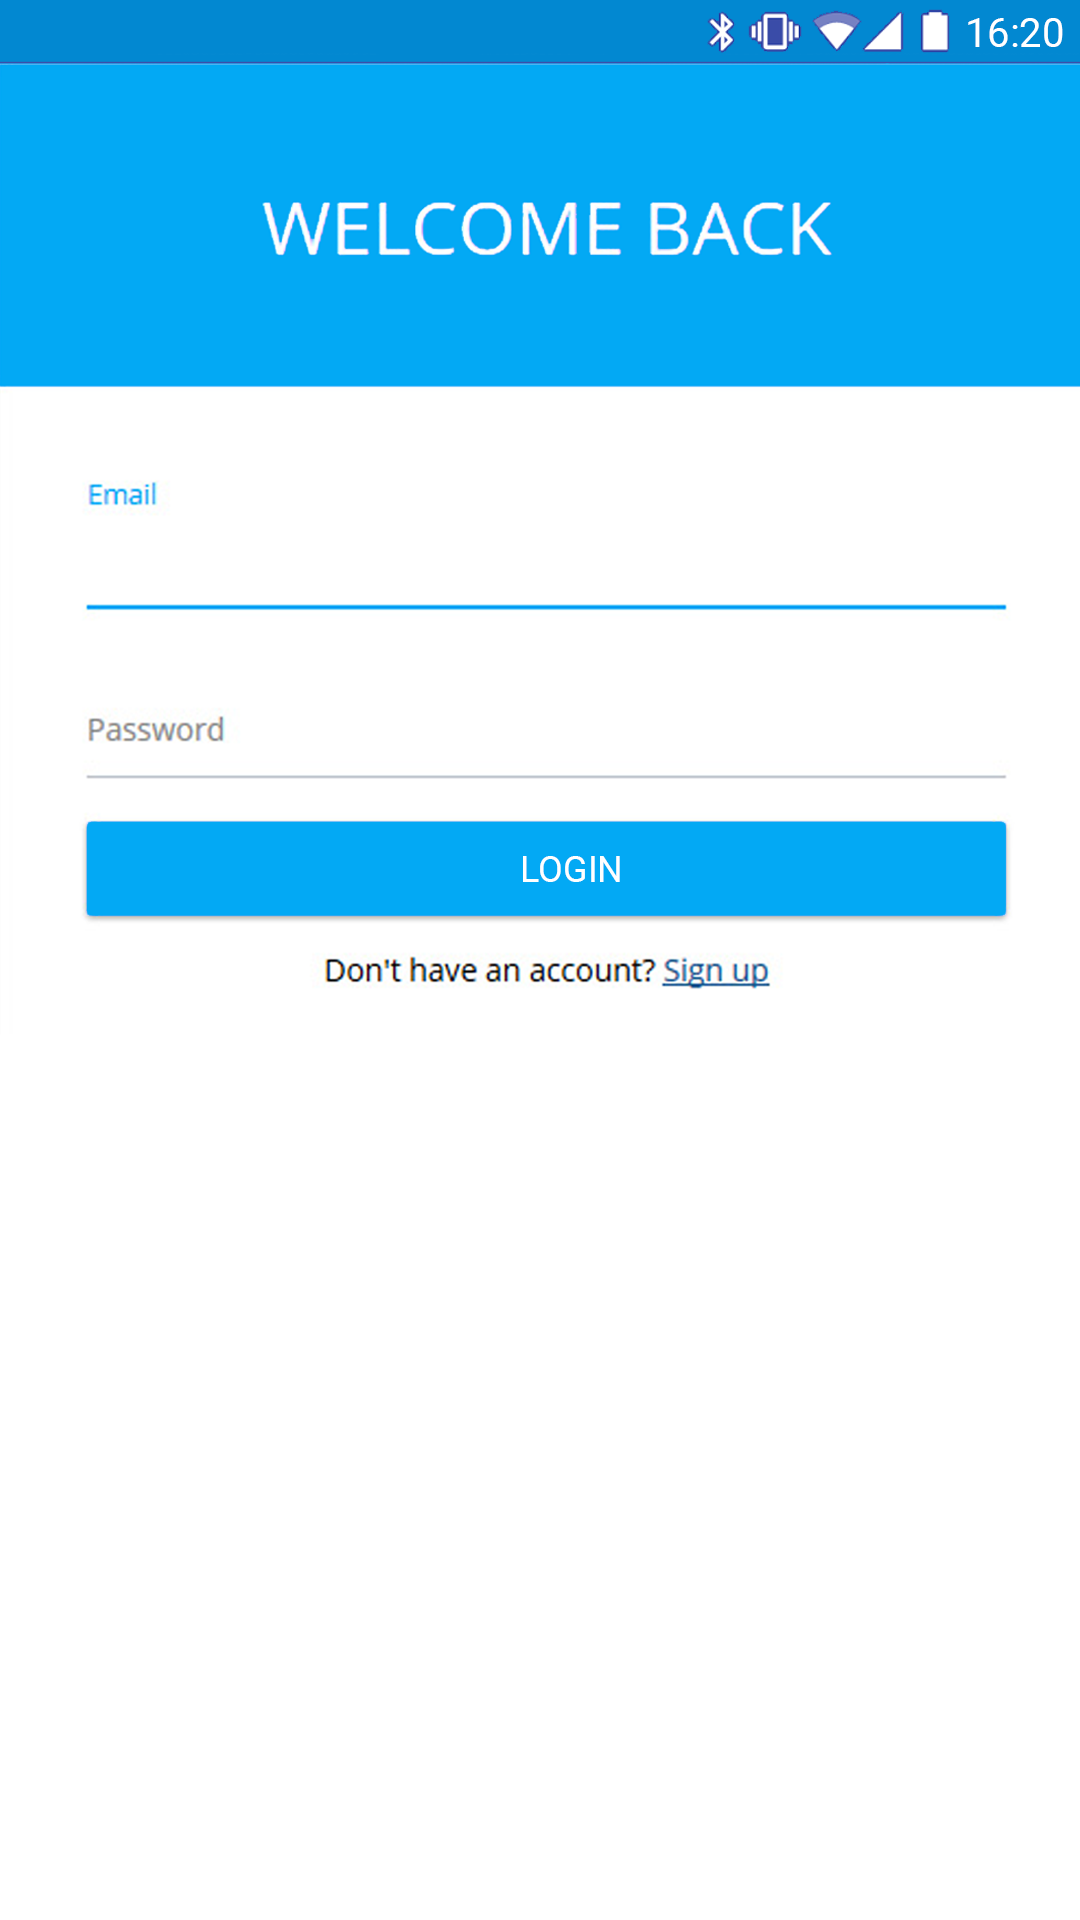
\includegraphics[width=0.9\linewidth]{manual/Login.png}
  \caption{\label{fig:vitals}The login screen}
\end{minipage}%
\begin{minipage}{.5\textwidth}
  \centering
  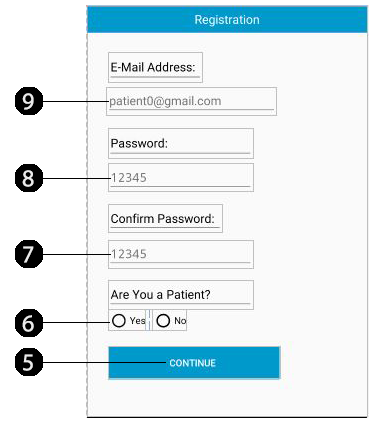
\includegraphics[width=0.9\linewidth]{manual/registration1.png}
  \caption{\label{fig:statistic}The registration screen 1}
\end{minipage}
\end{figure}


\begin{figure}[ht!]
\centering
\begin{minipage}{.5\textwidth}
  \centering
  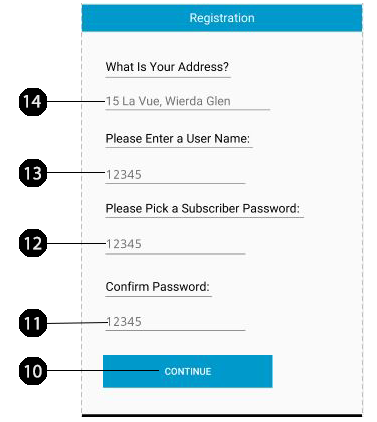
\includegraphics[width=0.9\linewidth]{manual/registration2.png}
  \caption{\label{fig:vitals}The registration screen 2}
\end{minipage}%
\begin{minipage}{.5\textwidth}
  \centering
  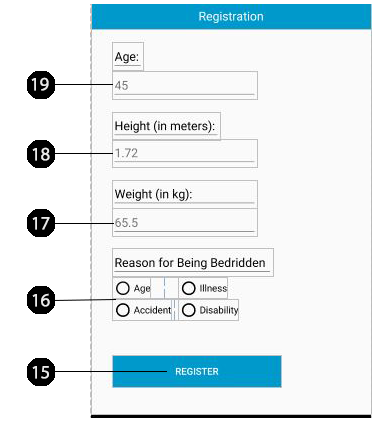
\includegraphics[width=0.9\linewidth]{manual/registration3.png}
  \caption{\label{fig:statistic}The registration screen 3}
\end{minipage}
\end{figure}

\begin{figure}[ht!]
\centering
\begin{minipage}{.5\textwidth}
  \centering
  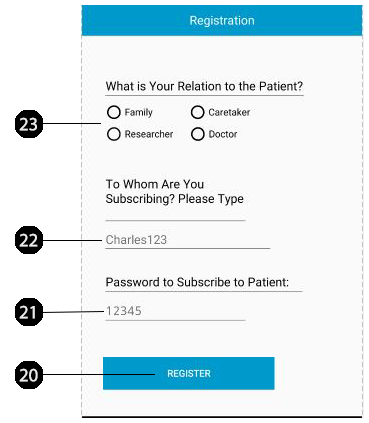
\includegraphics[width=0.9\linewidth]{manual/registration4.png}
  \caption{\label{fig:vitals}The registration screen 4}
\end{minipage}%
\begin{minipage}{.5\textwidth}
  \centering
  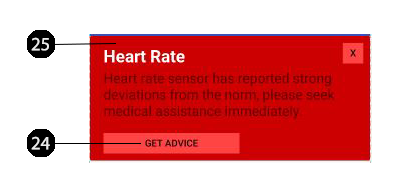
\includegraphics[width=0.9\linewidth]{manual/notification.png}
  \caption{\label{fig:statistic}The notifications screen}
\end{minipage}
\end{figure}

\begin{figure}[h!]
\centering
\begin{minipage}{.5\textwidth}
  \centering
  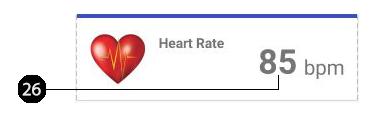
\includegraphics[width=0.9\linewidth]{manual/real-time.png}
  \caption{\label{fig:vitals}The real-time data screen 4}
\end{minipage}%
\begin{minipage}{.5\textwidth}
  \centering
  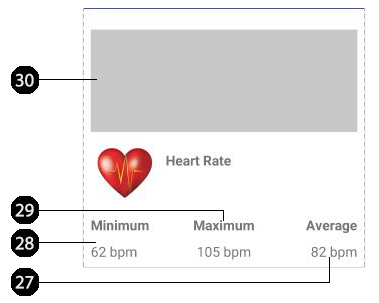
\includegraphics[width=0.9\linewidth]{manual/statistics.png}
  \caption{\label{fig:statistic}The statistics screen}
\end{minipage}
\end{figure}

\newpage
\pagebreak
\subsubsection{Main Login Screen (figure 1)}
\begin{enumerate}
   	\item The login button to be clicked once all necessary information has been filled out. 
   	\item The registration link that may be tapped in case users do not have an existing login. 
 	\item User password input section. (Needed for verification and validation before ReVA login). 
	\item User email address input section. (Used as a username to identify users). 
\end{enumerate}
\subsubsection{First Page of Registration (figure 2)}
NOTE: used by both subscribers and patients
\begin{enumerate}
\setcounter{enumi}{4}
	\item The continue button to proceed with the registration. 
	\item Yes/No radio button input to decide whether the user is a patient or subscriber. 
	\item Password confirmation input. 
	\item Password input for password that will be used for user login. 
	\item Email input for the email that will be used for user login. 
\end{enumerate}
\subsubsection{Second Page of Registration (figure 3)}
NOTE: meant only for patients
\begin{enumerate}
\setcounter{enumi}{9}
	\item The continue button for patients to proceed with the registration process. 
	\item Confirm password input for subscriber password. 
	\item Subscriber password input. (Will be used to verify and validate users wishing to subscribe to current patient). 
	\item Username input. (Will be used to identify patients). 
	\item Address input. (Stored in case of serious emergencies). 
\end{enumerate}
\subsubsection{Third Page of Registration (figure 4)}
NOTE: meant only for patients
\begin{enumerate}
\setcounter{enumi}{14}
	\item Register button. (Registers patient that has filled in all necessary information). 
	\item Bedridden reason radio input section. (Used to store the reason for patient being bedridden). 
	\item Weight input. (Used for measuring patient vitals more accurately). 
	\item Height input. (Used for measuring patient vitals more accurately). 
	\item Age input. (Used for measuring patient vitals more accurately). 
\end{enumerate}
\subsubsection{Fourth Page of Registration (figure 5)}
NOTE: meant only for subscribers (see description section)
\begin{enumerate}
\setcounter{enumi}{19}
	\item Register button for registering a subscriber. 
	\item Password to subscribe input. (Used to verify and validate subscriber). 
	\item Patient subscribing input. (Used to determine patient to which user wishes to subscribe). 
	\item Relation to patient input. (Used to determine the relation the subscriber has to the patient). 
\end{enumerate}
\subsubsection{Notification Alerts (figure 6)}
\begin{enumerate}
\setcounter{enumi}{23}
	\item Notification alert with title describing what vital it is reporting on and the description about what has gone wrong. 
	\item Advice button. (Used when user wishes to get advice about the notification).   
\end{enumerate}
\subsubsection{Real Time Data Screen (figure 7)}
NOTE:  Displays real time vitals data represented by an icon, a tag and a value.
\begin{enumerate}
\setcounter{enumi}{25}
	\item The current real time value of the vital beig monitored. 
\end{enumerate}

\subsubsection{Statistics and History Screen (figure 8)}
NOTE: . Displays statistical and historical vitals information in the form of a graph as well as minimum, maximum and average values for the vitals.
\begin{enumerate}
\setcounter{enumi}{26}
	\item The average value of the vital. 
	\item The minimum value of the vital. 
	\item The maximum value of the vital. 
	\item The graph representing the historical data of the vital. 
\end{enumerate}
